\documentclass[a4paper]{article}

%% Language and font encodings
\usepackage[english]{babel}
\usepackage[utf8x]{inputenc}
\usepackage[T1]{fontenc}

%% Sets page size and margins
\usepackage[a4paper,top=3cm,bottom=2cm,left=3cm,right=3cm,marginparwidth=1.75cm]{geometry}

%% Useful packages
\usepackage{amsmath}
\usepackage{graphicx}
\usepackage[colorinlistoftodos]{todonotes}
\usepackage[colorlinks=true, allcolors=blue]{hyperref}

\title{CS 6000 Journal Week 1}
\author{David Stout}

\begin{document}
\maketitle

\begin{abstract}
This paper is the beginning of the weekly journals for CS 6000-001 for the University of Colorado Colorado 
Springs. In this paper I will be talking a bit about the goals that I have for this class, what I hope to 
learn, my prospective degree track, and a little bit about me personally. 
\end{abstract}

\section{Goals for the course}

Coming into this course I was a little intimidated by the perceived complexity, but after Monday’s initial
lecture I feel very excited at the prospect of gaining confidence and experience in the art of research and writing research papers. I would like to learn about all the different techniques and methods used in the
varying fields of research, specifically computer science research, so that I am able to utilize the best
methods for my current and future research projects. Also, I am looking forward to being able to
effectively read and evaluate research papers, to determine their potential merit. I think that it will be 
very interesting to see what exactly makes a research paper publishable, and what journals are credible and 
reliable for publications to be taken seriously. It is my hope that I can utilize what I learn in this
class to be an effective researcher and later to be the best doctoral candidate that I can be.

I graduated in Fall 2017 with my Bachelors in Computer Engineering from the University of Colorado Colorado
Springs, and am currently working towards my PhD in Computer Science Engineering. My main areas of research are 
Software Engineering and Software Testing. Engineering and testing are very important for developers since 
engineering brings new innovations into the fold and testing allows for increased maintainability of the 
software development life cycle.

I like to relax by driving my motorcycle through the mountains, crafting retro gaming consoles from embedded 
systems, and scuba diving in the Caribbean.

\begin{figure}
\centering
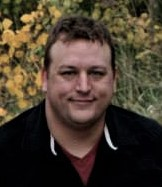
\includegraphics[width=0.3\textwidth]{profile2.jpg}
\caption{\label{fig:Me}This is a picture of me.}
\end{figure}

\section{Git repository location and learning this week}

\subsection{GitHub repository location with source code}

The GitHub repository that I have used is the one that I have created under the boultclass group, I plan to use 
this repo for all the assignments for this course.

The repo for this assignment may be found at:


\subsection{What I have learned this week}

This week, I have been focusing on learning the necessary tools to do the homework for this class. I had very limited exposure to LaTex previously and have never used Overleaf before, also I had never heard of Zotero and had to learn how to use it to my benefit.

\subsubsection{Problems and struggles that were overcome}


\subsection{How to write Mathematics}

\LaTeX{} is great at typesetting mathematics. Let $X_1, X_2, \ldots, X_n$ be a sequence of independent and identically distributed random variables with $\text{E}[X_i] = \mu$ and $\text{Var}[X_i] = \sigma^2 < \infty$, and let
\[S_n = \frac{X_1 + X_2 + \cdots + X_n}{n}
      = \frac{1}{n}\sum_{i}^{n} X_i\]
denote their mean. Then as $n$ approaches infinity, the random variables $\sqrt{n}(S_n - \mu)$ converge in distribution to a normal $\mathcal{N}(0, \sigma^2)$.


\subsection{How to create Sections and Subsections}

Use section and subsections to organize your document. Simply use the section and subsection buttons in the toolbar to create them, and we'll handle all the formatting and numbering automatically.

\subsection{How to add Lists}

You can make lists with automatic numbering \dots

\begin{enumerate}
\item Like this,
\item and like this.
\end{enumerate}
\dots or bullet points \dots
\begin{itemize}
\item Like this,
\item and like this.
\end{itemize}

\subsection{How to add Citations and a References List}

You can upload a \verb|.bib| file containing your BibTeX entries, created with JabRef; or import your \href{https://www.overleaf.com/blog/184}{Mendeley}, CiteULike or Zotero library as a \verb|.bib| file. You can then cite entries from it, like this: \cite{greenwade93}. Just remember to specify a bibliography style, as well as the filename of the \verb|.bib|.

You can find a \href{https://www.overleaf.com/help/97-how-to-include-a-bibliography-using-bibtex}{video tutorial here} to learn more about BibTeX.

We hope you find Overleaf useful, and please let us know if you have any feedback using the help menu above --- or use the contact form at \url{https://www.overleaf.com/contact}!

\bibliographystyle{alpha}
\bibliography{sample}

\end{document}